% !TeX program = pdflatex
% B subseteq A; C is not a subset of A; aspect and palette match GOLDEN SVG.
\documentclass[tikz,border=0pt]{standalone}
\usepackage{tikz}
\definecolor{DiagramInk}{HTML}{111111}
\definecolor{DiagramDash}{HTML}{555555}
\definecolor{DiagramGray}{HTML}{E9E9E9}
\begin{document}
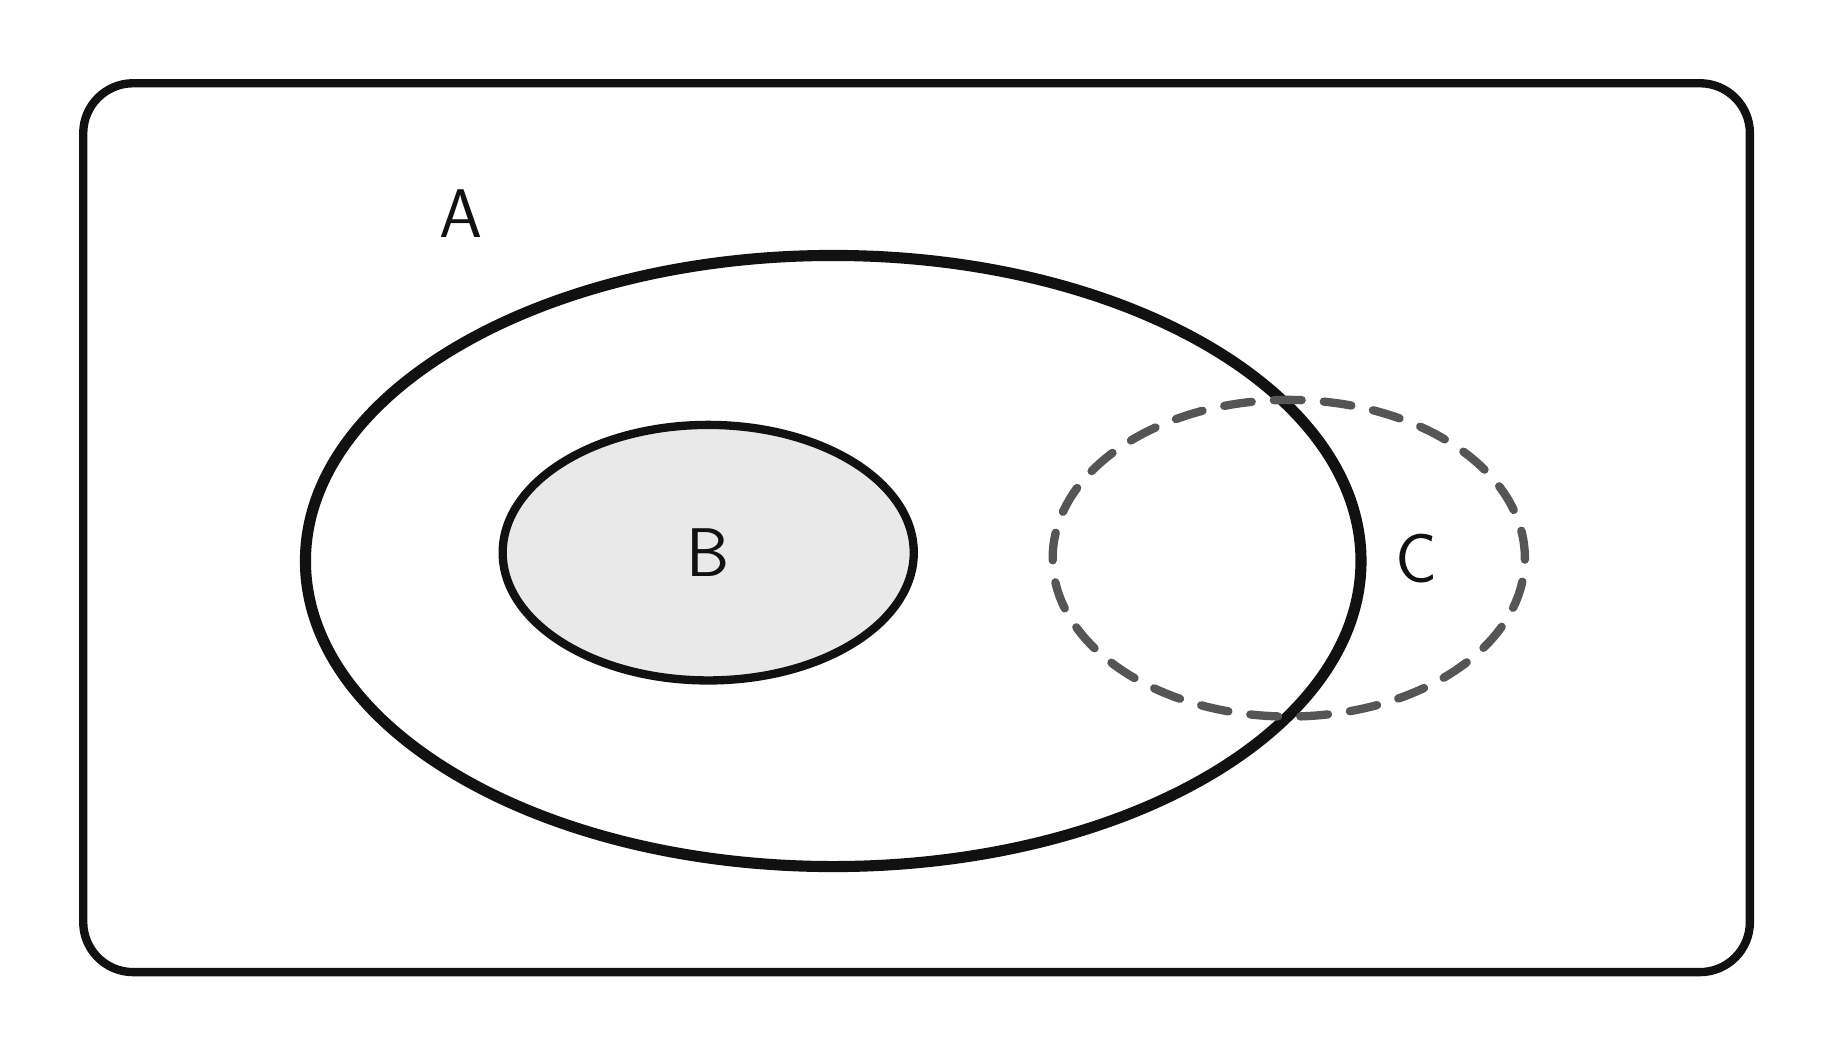
\begin{tikzpicture}[x=1bp,y=-1bp,line cap=round,line join=round]
  \path[use as bounding box] (0,0) rectangle (640,360);
  \fill[white] (0,0) rectangle (640,360);
  \draw[draw=DiagramInk,line width=3bp,rounded corners=18bp] (20,20) rectangle (620,340);
  \draw[DiagramInk,line width=4bp] (290,192) ellipse [x radius=190bp,y radius=110bp];
  \filldraw[fill=DiagramGray,draw=DiagramInk,line width=3bp] (245,189) ellipse [x radius=74bp,y radius=46bp];
  \draw[DiagramDash,line width=3bp,dash pattern=on 10bp off 8bp] (454,191) ellipse [x radius=85bp,y radius=57bp];
  \node[inner sep=0,anchor=center,text=DiagramInk,font=\sffamily\fontsize{32}{38}\selectfont] at (156,67) {A};
  \node[inner sep=0,anchor=center,text=DiagramInk,font=\sffamily\fontsize{30}{36}\selectfont] at (245,189) {B};
  \node[inner sep=0,anchor=center,text=DiagramInk,font=\sffamily\fontsize{30}{36}\selectfont] at (500,191) {C};
\end{tikzpicture}
\end{document}
